\subsection{Aktorik und Sensorik}
Die Aktorik des Würfels setzt sich aus den Bauteilen zusammen, welche bereits im 1D-Modell verwendet wurden. Allerdings sind drei Schwungmassen verbaut, womit auch drei Motoren bzw. Bremsen erforderlich sind.

\begin{figure}[!h]
\centering
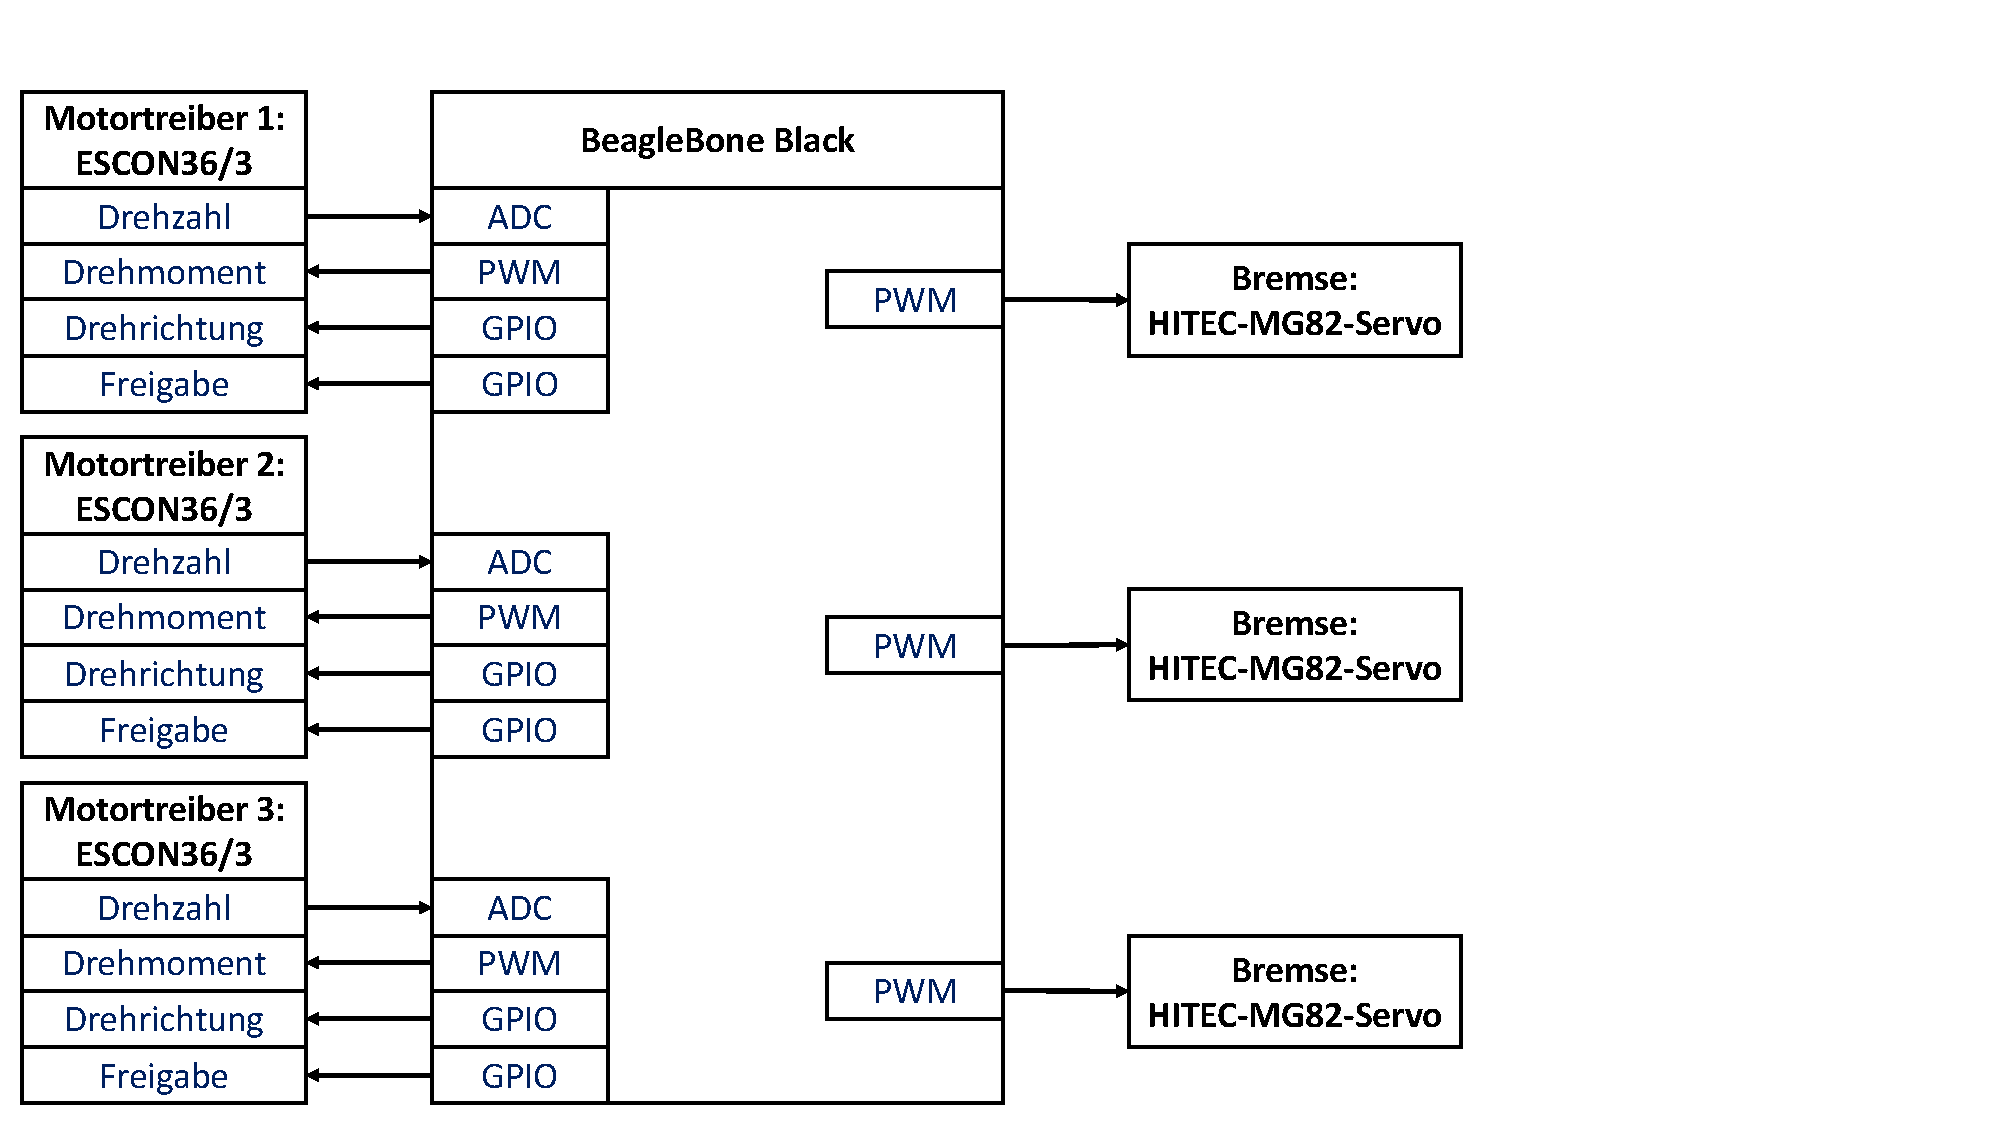
\includegraphics[width=0.8\linewidth, trim={0cm 0cm 7.5cm 1cm}, clip]{img/3D_AktorikBSB}
\caption{Übersicht Aktorik, Quelle: eigene Darstellung}
\end{figure}

Um die Position und Orientierung des Würfels im Raum zu bestimmen sind insgesamt sechs Sensoren nötigt. Die hier verwendeten GYR-521-Platinen können lediglich auf zwei verschiedene Adressen konfiguriert werden. Deshalb sind mehrere I2C-Bussysteme erforderlich. Da das BeagleBone Black lediglich zwei solcher Bussysteme zur Verfügung stellt wird ein analoger Switch verwendet um die Bussysteme der Sensoren sequenziell anzusteuern. Die Auswahl des Zielbusses wird mit Hilfe von digitalen Ausgängen festgelegt.

\begin{figure}[!h]
\centering
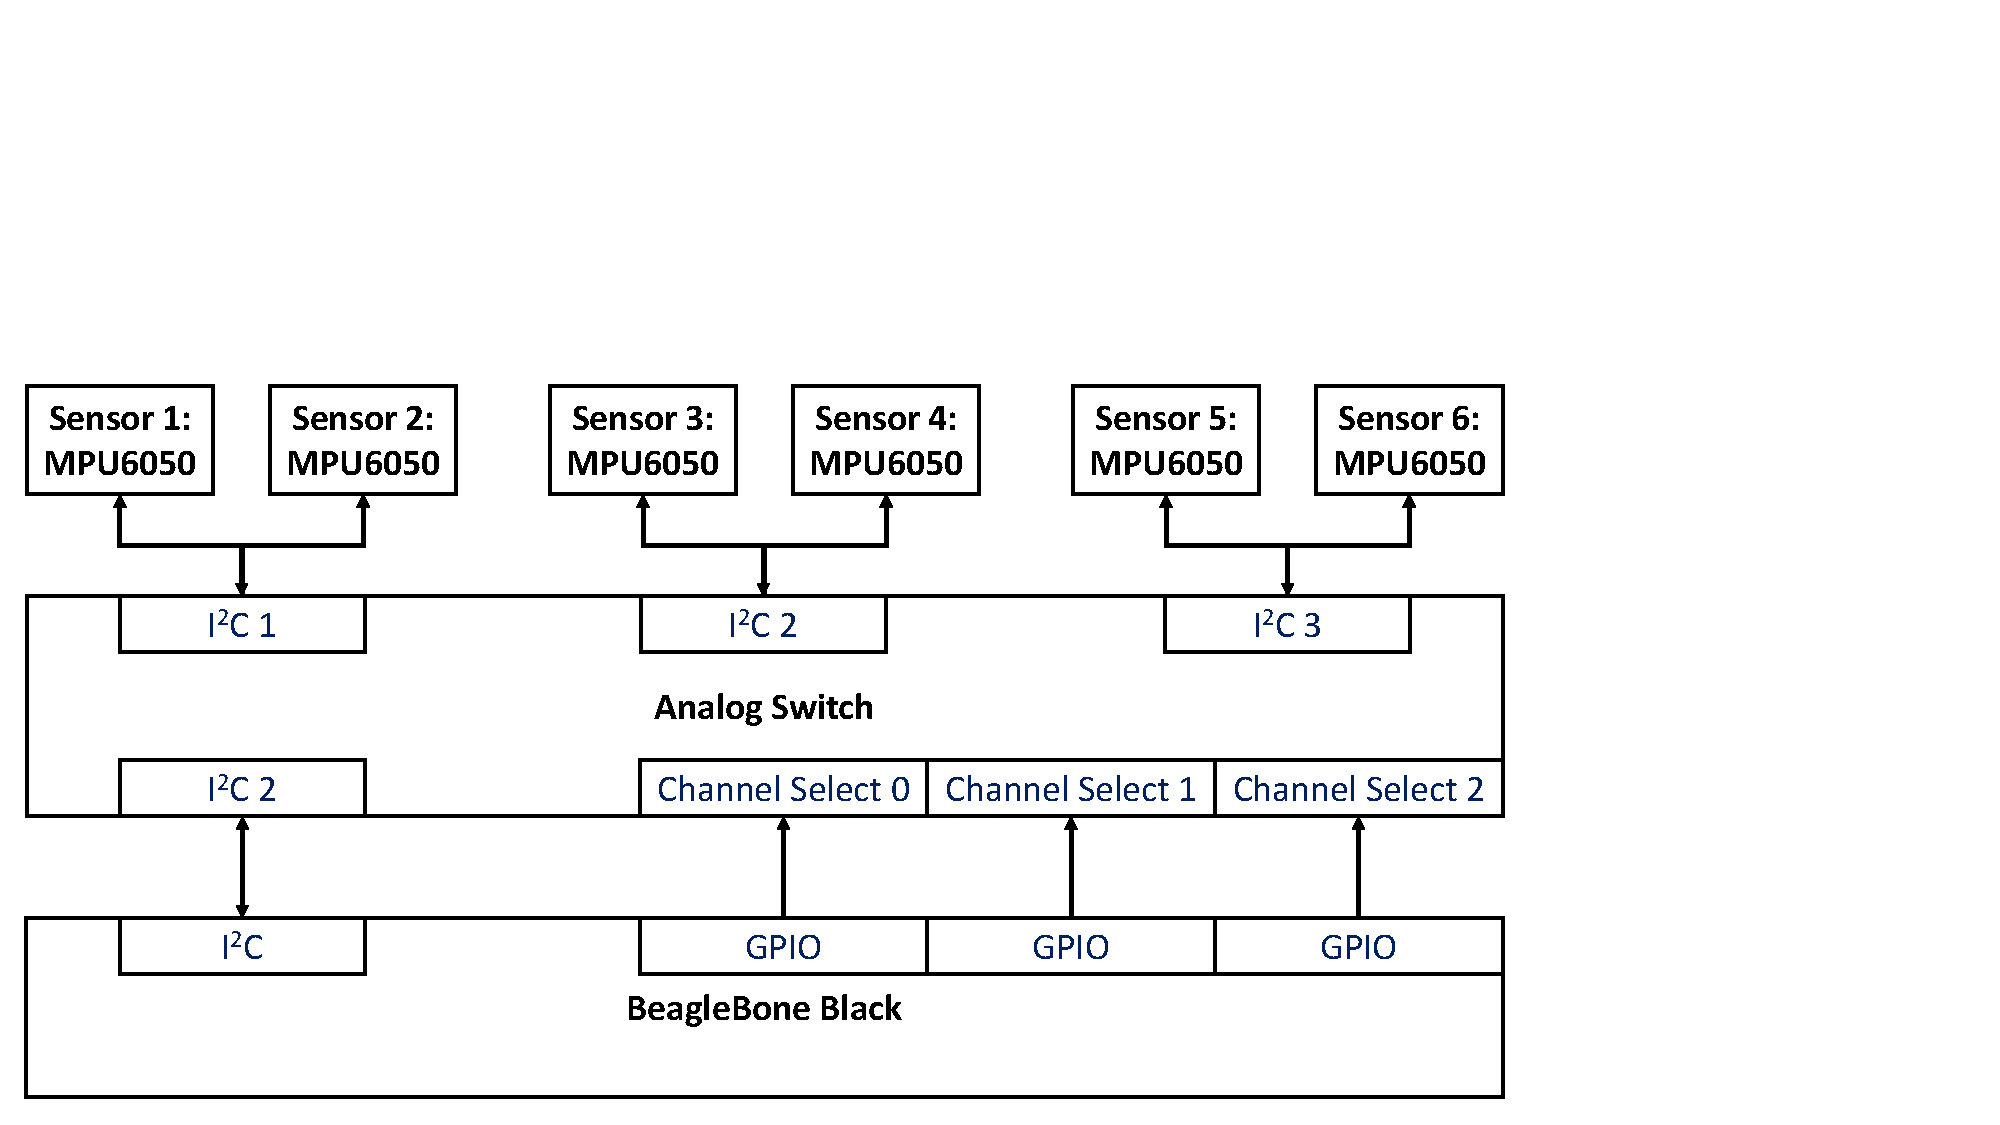
\includegraphics[width=0.8\linewidth, trim={0cm 0cm 8cm 6cm}, clip]{img/3D_SensorikBSB}
\caption{Übersicht Sensorik, Quelle: eigene Darstellung}
\end{figure}